%General
\documentclass{article}
\usepackage[utf8]{inputenc}
\usepackage{fullpage}

%Symbols
\usepackage{commath}
\usepackage{amsmath}
\usepackage{amssymb}
\usepackage{tikz}
\usetikzlibrary{arrows,automata}

%Formatting
\usepackage{bussproofs}
\usepackage{hyperref}
\usepackage{amsthm}
\usepackage{alltt}
\newtheorem{theorem}{Theorem}[section]
\newtheorem{definition}[theorem]{Definition}
\newtheorem{example}[theorem]{Example}
\hypersetup{colorlinks=true}
\hypersetup{colorlinks=true}
\usepackage{graphicx}
\graphicspath{ {img/} }
\usepackage{caption}

\title{Assignment 2: DFA and NFA}
\date{\today}
\author{Rikard Hjort}

\begin{document}
\maketitle

\section*{Problem 1}

The given automaton reaches has only one final state. When it reaches it, it stays there forever. This is symptomatic of an automata that accepts words that \textit{contain} certain sequences of symbols.

In this case, the automaton will not be affected by any number of $a$'s or $c$'s to begin with, but will transition to a new state when a $b$ is encountered. If another $b$ is encountered, it transtions back, so any sequence of $a$'s and $c$'s followed by two $b$'s will not affect the automaton. This can go on indeffinetly, so word beginning with pairs of $b$'s with any number of $a$'s and $c$'s \textit{between} the pairs will, after that beginning is processed, be in the initial state. When in state $q_1$, any number of $a$'s encountered will not affect the state, but as soon as a $c$ is encountered, the automaton will transition to an final state and stay there forever.

To transition to the final state, the automaton must encounter, at some point, an odd number of $b$'s, followed by any number of $a$'s, followed by a $c$.

\subsection*{Conclusion}

The automaton accepts the language over $\set{a,b,c}$ that contains all words which contain a sequence of an odd number of $b$'s, where that sequence has no neighbouring $b$'s\footnote{For example, the word $bbbc$ contains three sequneces of individual $b$'s which are odd, but also surrounded by other $b$'s. However, it also contains a sequence of three $b$'s which is odd, and has no surrounding $b$'s, so this word fulfills that criteria, whereas $bbc$ does not.}, followed by any number of $a$'s, followed by $c$.

\newpage
\section*{Problem 2}

\renewcommand{\labelenumi}{(\alph{enumi})}
\begin{enumerate}
        % a)
    \item 
        If the first symbol is not 0, we transition to the dead state. From there, whenever we encounter a 1, we go to an final state, and whenever we encounter a 0 to a non-final state. Thus, when the automaton has processed a word, it will be in an final state only if it passed the first test (begin with 0) and the last symbol processed was a 1.        

        The DFA is shown below with both table and diagram.
        \begin{align*}
            \begin{array}{r || c | c}
             & 0 & 1 \\ \hline
             \to q_0 & q_2 & q_1 \\ 
                q_1 & - & - \\
                q_2 & q_2 & q_3 \\
                *q_3 & q_2 & q_3
            \end{array}
        \end{align*}

        \begin{center}
        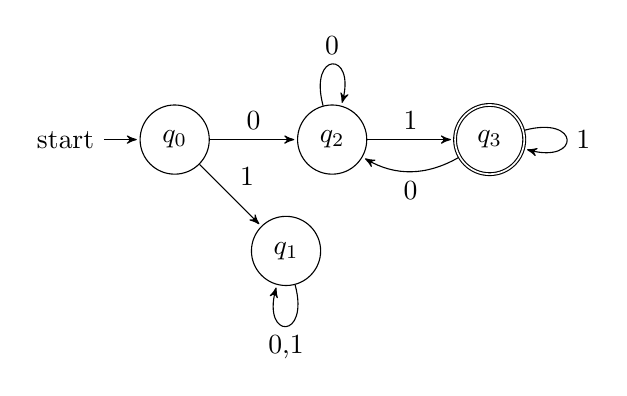
\begin{tikzpicture}[>=stealth',shorten >=1pt,auto,node distance=2cm]
            \node[initial, state]   (q0)    {$q_0$};
            \node[state]            (q1) [below right of=q0]    {$q_1$};
            \node[state]            (q2) [right of=q0]    {$q_2$};
            \node[state, accepting] (q3) [right of=q2]    {$q_3$};

            \path[->]
                (q0) edge node {1} (q1)
                     edge   node {0} (q2)
                 (q1) edge  [loop below] node {0,1} (q1)
                 (q2) edge  node {1} (q3)
                     edge   [loop above] node {0} (q2)
                 (q3) edge  [loop right] node {1} (q3)
                 edge [bend left] node {0} (q2);
        \end{tikzpicture}
        \end{center}

        % b)
    \item
        We let all state be final, except for one which is a dead state, representing that 110 was encountered.

        \begin{align*}
            \begin{array}{r || c | c}
                         & 0   & 1 \\ \hline
                \to *p_0 & p_0 & p_1 \\
                    *p_1 & p_0 & p_2 \\
                    *p_2 & p_3 & p_2 \\
                     p_3 & -   & -
            \end{array}
        \end{align*}

        $p_0$ remembers no 1's have been seen as the last character, $p_1$ remembers that exaclty one conseputive 1 has been seen, $p_2$ remebers two or more 1's have just been seen conseputively, and $p_3$ remembers that 110 has been seen at some point.

        % c)
    \item
        The product automaton $D= \set{Q,\Sigma, \delta,q_{00}, F}$ is the product of the two previous atomata. In the notation of $D$, let $s_{ij}$ be the state which $D$ is in after reading word $w$ if the first automaton would be in state $q_i$ after reading $w$ and the second automaton would be in state $p_j$. That is, in the notation below $s_{ij}$ is thought to be shorthand for $(q_i, p_j)$.

        We give the transition table for $D$.

        \begin{align*}
            \begin{array}{r || c | c}
             & 0 & 1  \\ \hline
                \to s_{00} & s_{20} & s_{11} \\
                s_{20} & s_{20} & s_{31} \\
                s_{11} & s_{10} & s_{12} \\
               *s_{31} & s_{20} & s_{32} \\
                s_{12} & s_{13} & s_{12} \\
                s_{10} & s_{10} & s_{11} \\
               *s_{32} & s_{23} & s_{32} \\
                s_{13} & - & - \\
                s_{23} & s_{23} & s_{33} \\
                s_{33} & s_{23} & s_{33}
            \end{array}            
        \end{align*}

        We see that for any row in the table, the transition from $s_{ij}$ to $s_{kl}$ happens iff the same input would transition the first automaton from $q_i$ to $q_k$ and the second automaton from $p_j$ to $p_l$.

        It is important to note that we give only 9 states in this table, even though the automaton actually has 16 state, one for each element in the set $\set{q_0,q_1,q_2,q_3} \times \set{p_0,p_1,p_2,p_3}$. However, only 9 sets are reachable, as only 9 states show up in the gradual construction of every possible state after reading a certain word. The unreachable states of course have their own transitions, but we omit them for clarity.
        
        %d)
    \item
        The DFA $D$ accepts a words only if it would be accpeted by the first and second automata in this problem. That is, it accepts the language over $\Sigma$ that contains all words which begin in 0, end in 1, and conatins no subword which is 110.
        % f)
    \item
        If we used the alternative product construction, the final states would be all which represent the first automaton being in a final state \textit{or} the second automaton being in a final state. That is, any state on the form $s_{i0}, s_{i1}, s_{i2}$ or $s_{3i}$ where $i$ is any number from 0 to 3. In the set of all states of $D$, the final states are

        $$\set{s_{00},s_{10},s_{20}, s_{30}, s_{01},s_{11},s_{21},s_{31}, s_{02},s_{12},s_{22},s_{32},s_{33}}$$
 
        However, not all of these are reachable! By cross-referencing the set above with the transition table we find that the reachable, final states are

        $$\set{s_{00},s_{10},s_{20}, s_{11}, s_{31}, s_{12},s_{32},s_{33}}$$

        The unreachable states that are still final are $\set{s_{21},s_{22}, s_{30}, s_{01}, s_{02}}$. If we look at them one by one, we see they are either $q_0$ combined with something else than $p_0$, which is impossible since we leave $q_0$ forever after reading the first symbol, or they represent a state $q_i$ which can only be reached by either 0 or 1, paired with a state $p_j$ which can only be reached by the \textit{other} symbol. $q_2$ can only be reached by reading a 0 while $p_1$ and $p_2$ are only reached by reading 1, and $q_3$ is only reached by 1 while $p_0$ is only reached by 0.

        %f)
    \item
        The DFA $D$ would accept the language over $\Sigma$ which containts all word words that

        \begin{itemize}
            \item starts in 0 and ends in 1, or
            \item does not contain the subword 110, or
            \item both of the above.
        \end{itemize}

\end{enumerate}

\newpage
\section*{Problem 3}

We begin by noting that $\epsilon$ will be accepted on both conditions: the word length and the amount of $a$'s plus the amount of $b$'s are both 0 in $\epsilon$, which means they are a multiple of 4 and even, respectively. Thus, the initial state should be final.

We construct two branches of the NFA. As soon as the first symbol is evaluated, the NFA jumps off inte both these branches, and never returns to the initial state.

One branch keeps track of the number of total symbols evaluated, modulo 4. It consists of 4 states, one of them accepting, and rotates between them to indicate the value modulo 4. The other branch of the NFA keeps track of the number of $a$'s and $b$'s encountered, modulo 2. This works in the same way, but only requires two states, and only transitions on the input $a$ or $b$. Where we start in this branch depends on the first symbol of the input.

Since we want to check if any of the conditions are true, we can treat the branches separately. If any of the conditions are true, the branch representing that condition will have "returned" to the initial state, meaning the word is accpeted, since one of the states the NFA is in after reading the word is the initial, final state.

The NFA is given with diagram and table below.

        \begin{center}
        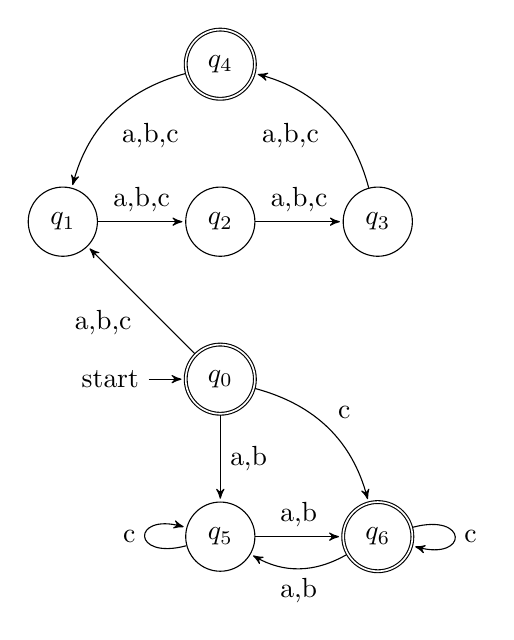
\begin{tikzpicture}[>=stealth',shorten >=1pt,auto,node distance=2cm]
            \node[initial, state, accepting]   (q0)    {$q_0$};
            \node[state]            (q2) [above of=q0]    {$q_2$};
            \node[state]            (q1) [left of=q2]    {$q_1$};
            \node[state] (q3) [right of=q2]    {$q_3$};
            \node[state, accepting] (q4) [above of=q2] {$q_4$};
            \node[state,] (q5) [below of=q0] {$q_5$};
            \node[state, accepting] (q6) [right of=q5] {$q_6$};

            \path[->]
                (q0) edge node {a,b,c} (q1)
                 (q1) edge node {a,b,c} (q2)
                 (q2) edge node {a,b,c} (q3)
                 (q3) edge [bend right] node {a,b,c} (q4)
                 (q4) edge [bend right] node {a,b,c} (q1)
                 (q0) edge node {a,b} (q5)
                    edge [bend left] node {c} (q6)
                 (q5) edge node {a,b} (q6)
                    edge [loop left] node {c} (q5)
                    (q6) edge [bend left] node {a,b} (q5)
                    edge [loop right] node {c} (q6)
                ;
        \end{tikzpicture}
        \end{center}

        \begin{align*}
            \begin{array}{r || l | l | l}
                & a & b & c  \\ \hline
                \to *q_0 & \set{q_1, q_5} & \set{q_1, q_5} & \set{q_1, q_6} \\
                q_1 & \set{q_2}& \set{q_2}& \set{q_2} \\
                q_2 & \set{q_3}& \set{q_3}& \set{q_3} \\
                q_3 & \set{q_4}& \set{q_4}& \set{q_4} \\
                *q_4 & \set{q_1}& \set{q_1}& \set{q_1} \\
                q_5 & \set{q_6}& \set{q_6}& \set{q_5} \\
                *q_6 & \set{q_5}& \set{q_5}& \set{q_6} \\
            \end{array}
        \end{align*}

        \subsection*{Constructing the DFA}

        We explore the possible subsets of the DFA incrementally, starting in the initial state, which is $\set{q_0}$. From there, we take unions of all the sets we can transition to from our current states to create unique subsets, representing the state of the DFA. We will add new subsets to the table as we discover them, which will determine the order int which they appear in the table.

        %shit, wrong
        \begin{align*}
            \begin{array}{r || l | l | l}
                & a & b & c \\ \hline
                \to *\set{q_0} & \set{q_1, q_5} & \set{q_1, q_5} & \set{q_1, q_6} \\
                \set{q_1, q_5} & \set{q_2, q_6} & \set{q_2,q_6} & \set{q_2, q_5} \\
                *\set{q_1, q_6} & \set{q_2, q_5} & \set{q_2,q_5} & \set{q_2, q_6} \\
                \set{q_2,q_5} & \set{q_3, q_6} & \set{q_3,q_6} & \set{q_3, q_5}  \\
                *\set{q_2,q_6} & \set{q_3, q_5} & \set{q_3,q_5} & \set{q_3, q_6}  \\
                \set{q_3,q_5} & \set{q_4, q_6} & \set{q_4,q_6} & \set{q_4, q_5}  \\
                *\set{q_3,q_6} & \set{q_4, q_5} & \set{q_4,q_5} & \set{q_4, q_6}  \\
                *\set{q_4,q_5} & \set{q_1, q_6} & \set{q_1,q_6} & \set{q_1, q_5}  \\
                *\set{q_4,q_6} & \set{q_1, q_5} & \set{q_1,q_5} & \set{q_1, q_6}
            \end{array}
        \end{align*}

        We show this automaton also with a diagram, where the node names are all the numbers $i$ for which $q_i$ is in the subset that node represents.

        
        \begin{center}
        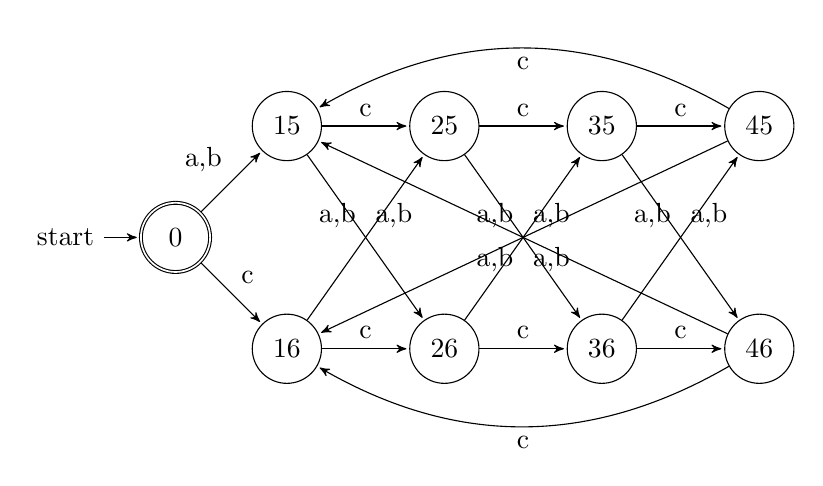
\begin{tikzpicture}[>=stealth',shorten >=1pt,auto,node distance=2cm]
            \node[initial, state, accepting]   (0)    {0};
            \node[state] (15) [above right of=0] {15};
            \node[state] (16) [below right of=0] {16};
            \node[state] (25) [right of=15]{25};
            \node[state] (26) [right of=16]{26};
            \node[state] (35) [right of=25]{35};
            \node[state] (36) [right of=26]{36};
            \node[state] (45) [right of=35]{45};
            \node[state] (46) [right of=36]{46};

            \path[->]
                (0) edge node {a,b} (15)
                    edge node {c} (16)
                (15) edge node {c} (25)
                    edge node {a,b} (26)
                (25) edge node {c} (35)
                    edge node {a,b} (36)
                (35) edge node {c} (45)
                    edge node {a,b} (46)
                (45) edge [bend right] node {c} (15)
                    edge node {a,b} (16)

                (16) edge node {c} (26)
                    edge node {a,b} (25)
                (26) edge node {c} (36)
                    edge node {a,b} (35)
                (36) edge node {c} (46)
                    edge node {a,b} (45)
                (46) edge [bend left] node {c} (16)
                    edge node {a,b} (15)
                ;
        \end{tikzpicture}
    \end{center}

    \end{document}
